\section{Fundamentals of Metal Oxide Semiconductor structures}
MOS structures are the basis for modern integrated circuits
\cita{sze_physics_2007}
which make up PCs, mobile devices and communication infrastructure.
The CMOS fabrication process which produces these structures
has enabled processing power to grow exponentially,
by steadily shrinking the transistors that make up an integrated circuit
(\figref{fig:moore}).
\fig{moore}{figuras/moore/moore.pdf}
{Exponential reduction in transistor size.
The number of transistors in a microprocessor doubles every two years,
following Moore's law
\cite{moore_cramming_2006}.
Reprinted from \cite{sedra_microelectronic_2010}.}
\subsection{MOS capacitor}
Before studying MOS transistors, it is necessary to understand MOS capacitors.
Fabrication begins with a ~\SI{1}{\milli\meter} silicon wafer cut from a monocrystalline ingot.
Its surface is oxidized in order to produce a thin insulating SiO$_2$ layer.
Both this step and subsequent treatment and annealing steps
determine a crucial property of the Si-SiO$_2$ interface:
the surface density of electronic states.
If this number is too large, the device characteristics are negatively impacted:
for example, through higher noise and parameter shifts over time.
The invention that improved interfaces and thus enabled decent MOS transistors
came decades after the MOS was originally patented
\cite{chih-tang_evolution_1988}.

On top of the oxide layer, a conductor (gate) is deposited,
as seen in \figref{fig:cortemos}.
This conductor can be polysilicon (polycrystalline silicon) or,
in recent processes, metal.
\fig{cortemos}{figuras/mos/corte.png}{Cross section of a MOS structure.
Reprinted from~\cite{sze_physics_2007}.}

This structure forms a capacitor, with two conductors separated by a dielectric.
%
\subsubsection{Band structure}
The following analysis assumes a MOS whose dimensions along the wafer
are much larger than the characteristic distance 
across which the electric field varies normal to the wafer.
This allows us to use a 1D model,
neglecting field variations parallel to the wafer.

The ideal MOS band structure is depicted in \figref{fig:bandasmos}.
An ideal MOS has no charge trapped in the oxide nor in the oxide-semiconductor interface.
Therefore, its bands are flat under zero bias.
We will analyze how band position varies with applied bias and with distance from the wafer surface.

When a voltage source (eg. a battery) is connected across the terminals,
it fixes the difference between the Fermi levels of the metal and the semiconductor.
The resulting $E_F$ gradient leads to a current within the MOS which restores equilibrium
(\figref{fig:polarizacionmos}).

%Bajo la condición $V=0$, los niveles de Fermi de metal y
%semiconductor coinciden.
%Para cada material, el nivel de vacío $\phi$ 
%está a una distancia fija del nivel de Fermi.
%En un metal esta distancia se denomina función trabajo.
%En un semiconductor esta cantidad es la suma de la afinidad electrónica $\xi$
%(distancia entre la banda de conducción y el nivel de vacío)
%y 
%Por ejemplo, la función trabajo del aluminio es \SI{4.2}{\volt} y la de una
%oblea dopada tipo P típica es \SI{3.6}{\volt}.
%Cuando coinciden los niveles de Fermi de metal y semiconductor, 
%difiere su potencial eléctrico en \SI{0.6}{\volt}.
%$\phi$ varía de forma contínua entre las terminales,
%curvando las bandas.
%Hace falta aplicar una tensión $V_{fb}=(\phi_m-\phi_s)/e$ 
%para obtener bandas planas (que implican, por Poisson, carga nula).
%
\fig{bandasmos}{figuras/mos/bandas.png}
{Band structure of a MOS capacitor in the flatband condition.
Reprinted from~\cite{sze_physics_2007}.}
\begin{figure}[H]
    \centering
    \begin{subfigure}[b]{.3\textwidth}
        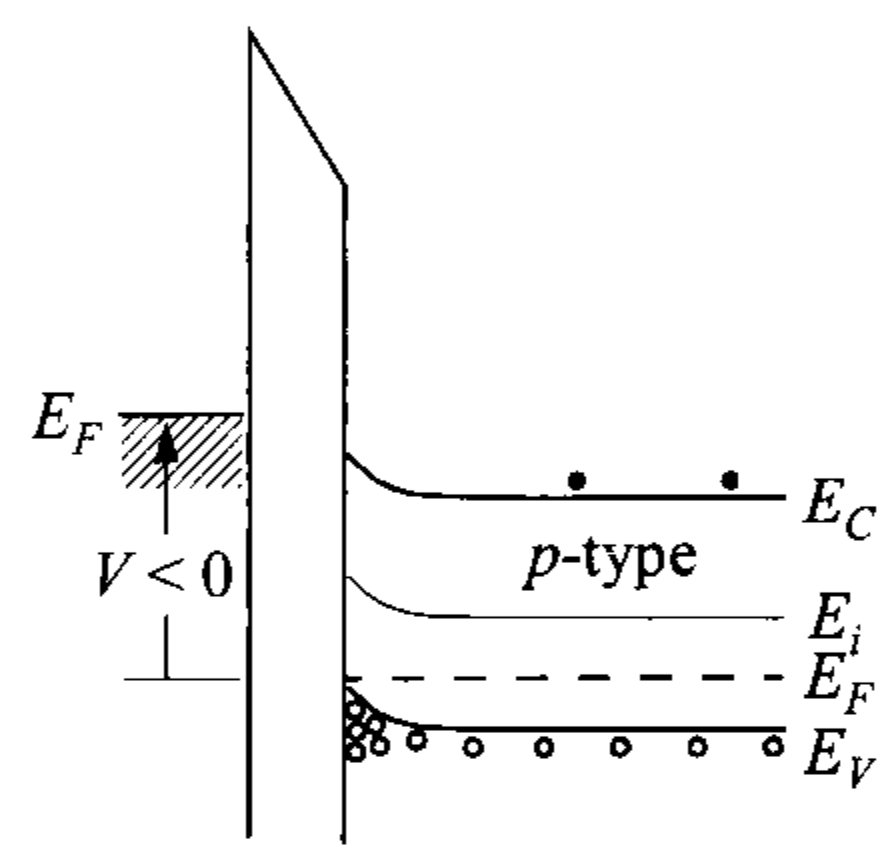
\includegraphics{figuras/mos/acumulacion.png}
        \label{fig:mosacumulacion}
        \caption{Accumulation}
    \end{subfigure}
    \begin{subfigure}[b]{.3\textwidth}
        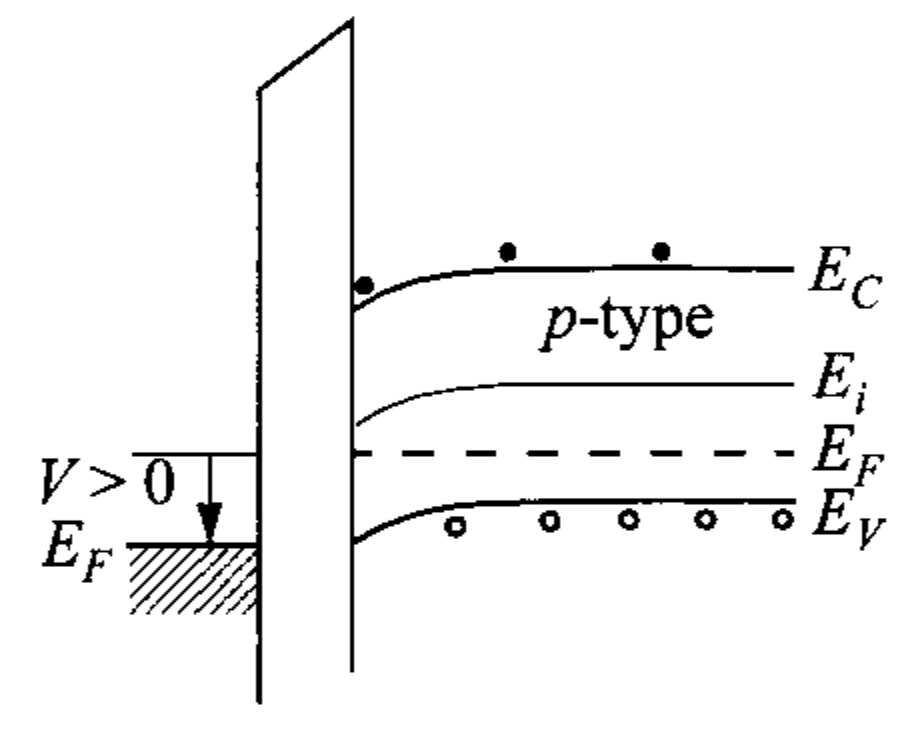
\includegraphics{figuras/mos/desercion.png}
        \label{fig:mosdesercion}
        \caption{Depletion}
    \end{subfigure}
    \begin{subfigure}[b]{.3\textwidth}
        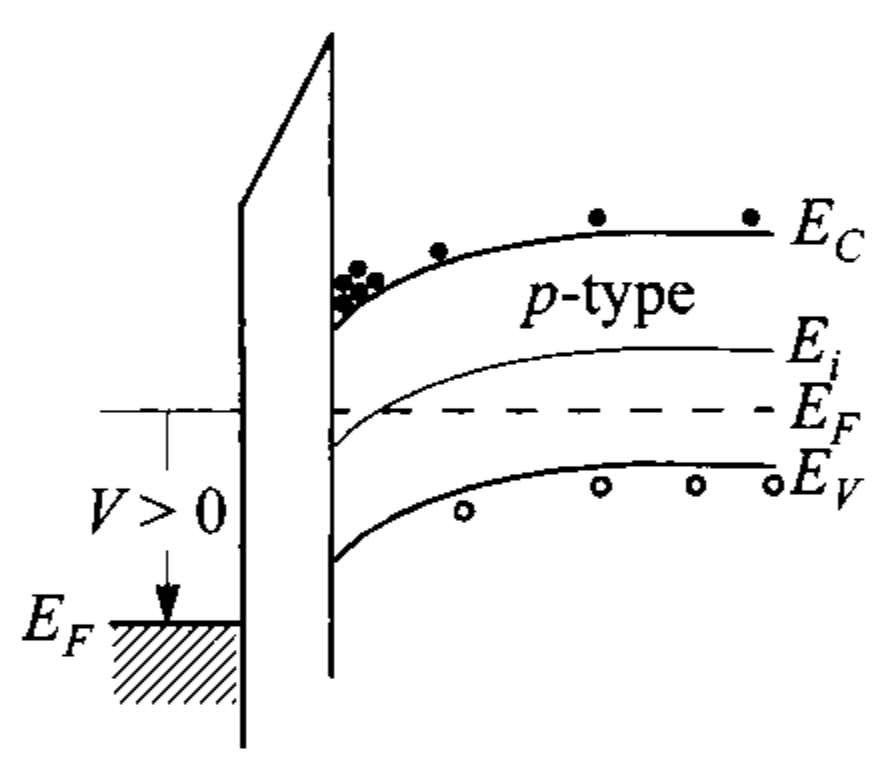
\includegraphics{figuras/mos/inversion.png}
        \caption{Inversion}
        \label{fig:mosinversion}
    \end{subfigure}
    \caption{Band structure of a MOS under bias, for $V_{fb}=0$.
Reprinted from~\cite{sze_physics_2007}.}
    \label{fig:polarizacionmos}
\end{figure}
%
\subsubsection{Carrier concentration}
In order to model electron and hole concentration in semiconductors,
one starts from the independent electron approximation.
This means considering one-electron levels which are occupied by identical,
non-interacting electrons.
This type of system is described by Fermi-Dirac statistics,
which state that the probability that a level is occupied is given by
\begin{align*}
    f(E) = \left[\exp\left(\frac{E-E_F}{kT}\right)+1\right]^{-1}
\end{align*}
with $E$ the level energy and $E_F$ the fermi level.
$E_F$ is a constant throughout any system in chemical equilibrium,
and can be solved for as a function of the total number of particles.
This is done by inverting the equation $N=\sum_E f(E)$,
with the sum spanning all energy levels.

In order to calculate the average number of carriers in a band,
it is necessary to sum the occupancy of all the energy levels within it.
We can simplify this sum in the non-degenerate case, where
the conduction band is many thermal energies away from the Fermi level:
$|E-E_F| \gg kT$.
This allows us to approximate the Fermi-Dirac distribution using a
Maxwell-Boltzmann distribution:
\begin{align*}
    f(E) \approx \exp\left(-\frac{E-E_F}{kT}\right)
\end{align*}.
Moreover, the sum over energy levels can be approximated by an integral
over energy, leading to the following hole and electron concentrations:
\begin{align*}
    n_c = N_c(T)e^{-\frac{\epsilon_c-E_F}{k_BT}}\\
    p_v = P_v(T)e^{-\frac{E_F-\epsilon_v}{k_BT}}
\end{align*} with $N_c(T)$ y $P_v(T)$ two slowly-varying functions of temperature.

It is helpful to write the carrier concentration as a function of the bulk potential.
This is a distant reference point in the semiconductor, which we use as a reference:
$\psi_p=\phi(x)-\phi(\infty)$,
\begin{align}
    n &= n_0\exp\left(\frac{q\psi_p}{kT}\right)&
    p &= p_0\exp\left(-\frac{q\psi_p}{kT}\right),
    \label{eq:portadores_nodegenerados}
\end{align}
with $n_0$ and $p_0$ the bulk carrier concentrations.
\subsubsection{Doping}
A central part of the fabrication process is the introduction of dopants
which increase the number of holes or electrons in specific regions.
The geometry and dopant concentration of each region define what kinds of devices
can be created in a given process.
For example, a process might be designed for high voltages by using low concentrations
and large separations, which result in large junction breakdown voltages.

One doping technique is called Chemical Vapor Deposition.
It consists of exposing the wafer to a gas such that atoms diffuse from
the gas phase to the wafer.
Another technique is implanting: dopants are ionized and then accelerated
towards the wafer using electric field.
This allows the penetration depth to be controlled by varying the
acceleration energy
\cite{campbell_science_2001}.

The mechanism by which dopants add carriers is by capturing or emitting electrons.
This ionizes the impurity atom.
In order to model this phenomenon,
impurity atoms are modeled as though they were a normal Silicon lattice atom,
and an additional charge depending on its valence number
(+1 for pentavalent impurities like P, -1 for trivalent like B).
This additional charge can form bound electron states.
By using the effective mass equation\cite{datta_quantum_1989},
% FIXME: feo
one can conclude that the binding energy is typically very low.
Therefore, dopant atoms are almost completely ionized under normal temperature ranges.
This is due to the periodic Silicon lattice, which acts in two ways.
First, it is a dielectric which shields the dopant's electric field.
Second, it gives the electron a smaller effective mass,
which lowers the kinetic energy
(and therefore the potential energy, through the Virial theorem)

Typically, a region has more dopants of one kind than the other,
by several orders of magnitude.
It is then said that the holes or the electrons are the majority carrier.
It can also be said that the region is p-type (majority holes)
or n-type (majority electrons).

Under this condition, the majority carrier concentration is approximately equal
to its dopant concentration.
The minority carrier concentration is suppressed due to Le Chatelier's principle,
and is approximately equal to $n_i^2/N_a$ 
with $n_i$ the intrinsic (pure) carrier concentration for the semiconductor,
and $N_a$ the majority doping concentration.

\subsubsection{Charge-voltage relation}
Starting from Poisson's equation for the semiconductor potential $\phi$,
one reaches
\begin{align*}
    \deriv{^2\phi}{x^2} &= \frac e{\epsilon_s}(N_d-N_a+p-n),
\end{align*}
where the right-hand side terms are concentrations of donors, acceptors,
holes and electrons, respectively.

Approximation~\ref{eq:portadores_nodegenerados} is valid for the nondegenerate
condition
$|E_F-E_{c/v}|\gg kT$, 
meaning the Fermi level is several thermal energies away from the band edges.
This leads to a set of equations which we can solve for the electric field:
\begin{align*}
    \mathscr{E}_s &= \pm \frac{\sqrt 2kT}{qL_D}
    F(q\psi_p/kT,n_{p0}/p_{p0})\textnormal{, with}\\
    L_D^2&=\frac{kT\epsilon_s}{p_{p0}q^2}\textnormal{ , and}\\
    F(x,y) &= \sqrt{e^{-x}+x-1+y(e^x-x-1)}.
\end{align*}
Applying Gauss' law leads to the total charge in the semiconductor:
\begin{align*}
    Q_s = -\epsilon_s\mathscr{E}_s.
\end{align*}

We can find the relation between $V_G$ and $\psi_p$ by
using the voltage drop across the gate oxide,
and the continuity of the normal component of the displacement field:
\begin{align}
    V_G &= \psi_s + \mathscr{E}\frac{\epsilon_s}{\epsilon_{ox}}t_{ox}.
    \label{eq:potencial_campo_mos}
\end{align}
This yields the curve in \figref{fig:cargamos},
where one can highlight the operating regions.
%
\subsubsection{MOS capacitor operating regions}
\begin{itemize}
    \item Accumulation:
        When the gate is negatively biased,
        the semiconductor surface acquires additional majority carriers.
    \item Flatband:
        At zero gate voltage, the positive charge from the holes
        (portadores mayoritarios)
        cancels with the negative charge from the acceptor ions,
        leading to $Q=0$. 
    \item Depletion/weak inversion:
        With increasing gate voltage,
        the semiconductor surface is depleted of majority carriers.
        This leaves behind the negative charge from acceptor ions.
    \item Strong inversion:
        When the surface potential crosses $2\psi_B$,
        the surface is filled with minority electrons,
        with a concentration equaling that of majority carriers in the bulk.
        Additional increases in $\psi_s$ result in exponential growth in
        $|Q|$.
        This remains true until the Fermi level gets close to 
        the conduction band edge, which is called degeneracy.
        When this happens, the semiconductor behaves like a metal,
        whose carrier density varies very weakly with potential.
        Before this point is reached,
        charge grows linearly with $V_G$
        because most additional voltage is dropped across the gate oxide.
\end{itemize}
\fig{cargamos}{figuras/mos/carga_vg.pdf}{Charge in a typical MOS
    ($N_A=$\SI{4e15}{\centi\meter^{-3}}) as a function of gate voltage.
In the left of the graph, the Fermi level grows near to the valence band edge.
This breaks the nondegeneracy assumption, meaning that Fermi-Dirac statistics
must be used without approximation.}
%
%
\subsection{MOS transistor}
Transistors are the base of modern electronics.
By modulating one signal with another,
they implement analog operations like amplification and multiplication.
When used with discrete levels (on/off),
they implement the basic logic gates (NOT, AND, etc)
which combine to form a digital circuit.
Their steady improvement has allowed for a growing number of 
digital and analog functions
to be integrated in a single chip.
%
\subsubsection{Circuit model}
\label{section:ecuaciones_mos}
The MOSFET or MOS transistor is a 4-terminal device:
drain, gate, source and body (\figref{fig:mosfetschem}).
\fig{mosfetschem}{figuras/mos/mosfet.pdf}{Schematic symbol of the MOS transistor}
In many cases, the source is shorted to the body,
which breaks the drain-source symmetry.
The gate-source voltage controls the current from drain to source.

\Figref{fig:mosfetoutput} shows 3 operating regions for the MOSFET:
\fig{mosfetoutput}{figuras/mos/output.pdf}{Output characteristics of a MOSFET}
\begin{itemize}
    \item Cutoff: when $V_g<V_T$, no drain current flows.
        This is why $V_T$ is called the threshold voltage.
        $V_T$ is a parameter fixed by the fabrication process
        which is close to \SI{.3}{\volt} in modern CMOS processes.
        A more accurate model for this region is that $I_d$ varies
        exponentially with $V_gs$.
    \item Triode: when $V_g>V_T$ and $V_{ds}<V_g-V_T$, 
        drain current grows with drain-source voltage according to
        \begin{align*}
            I_D&=\beta_n\frac WL(V_{gs}-V_T-\frac{V_{ds}}2)V_{ds},
        \end{align*}
        with $\beta_n$ a parameter fixed by the fabrication process
        and $\frac WL$ the MOSFET's aspect ratio.
    \item Saturation: when $V_g>V_T$ and $V_{ds}>V_g-V_T$,
        drain current is approximately independent of $V_ds$:
        \begin{align*}
            I_{Dsat}&=\frac{\beta_n}2\frac WL(V_{gs}-V_T)^2.
        \end{align*}
\end{itemize}
%
\subsubsection{Physical modeling}
An N-channel MOSFET consists of a MOS capacitor on a p-type substrate
between two highly doped n-type regions.
These two regions form the drain and source (\figref{fig:mosfetestructura}).
In the absence of gate voltage,
no current can flow from drain to source because 
one of the p-n junctions (drain-substrate or source-substrate) is reverse-biased.

When the MOS is inverted,
a layer of electrons form a conduction channel near the surface of the silicon.
This n-type region connects the drain to the source, allowing for current to flow.
As gate voltage varies,
the variation of charge in the channel modulates its conductivity.
\fig{mosfetestructura}{figuras/mos/mosfet.png}{MOSFET structure.
Reprinted from~\cite{sze_physics_2007}.}
